\documentclass[11pt, addpoints, answers]{exam}

\usepackage{amsmath, amssymb}
\usepackage{xcolor}
\usepackage{tikz}
\usepackage{enumerate}
\usepackage{graphicx}
\usepackage{tabularx}

\newcommand{\red}[1]{\textcolor{red}{#1}}
\newcommand{\blue}[1]{\textcolor{blue}{#1}}
% For inserting code snippets.
\usepackage{listings}
\lstset{
    columns = fixed,
    basewidth = {0.5em},
    breaklines = true,
    backgroundcolor = \color{white},
    keywordstyle = \color[RGB]{40, 40, 255},
    numberstyle = \footnotesize\color{darkgray},
    commentstyle = \ttfamily\color{violet},
    basicstyle = \ttfamily,
    stringstyle = \ttfamily\color[RGB]{128, 0, 0},
    showstringspaces = false,
    language = {[11]C++},
    escapechar = \@
}
\lstnewenvironment{cpp}[1][]{\lstset{language = {[11]C++}, #1}}{}

\renewcommand{\baselinestretch}{1.15}
\setlength{\parskip}{1.25\baselineskip}

% headers, footers, titles
\newcommand{\CourseName}{CS101 Algorithms and Data Structures}
\newcommand{\HomeworkNO}{7}
\newcommand{\DueDate}{November 20, 2024} % TODO: REMEMBER TO MODIFY

\pagestyle{headandfoot}
\runningheadrule
\runningheader{CS101 24Fall}{Homework \HomeworkNO}{Due on: \DueDate}
\runningfooter{}{\thepage}{}

\title{
    \vspace{25pt}
    \LARGE ShanghaiTech University \\
    \bigskip
    \textbf{\CourseName} \\
    \textbf{Fall 2024}   \\
    \bigskip
    Homework \HomeworkNO
}
\author{}
\date{Due date: \DueDate, at 23:59}

% formats of questions, choices, points, etc.
\qformat{\bf\thequestion. (\totalpoints\ points) \thequestiontitle\hfill}
\pointname{'}
\SolutionEmphasis{\color{black}}
\CorrectChoiceEmphasis{\bf\color{blue}}



% We frequently use this font.
\newcommand{\dfuttt}{\texttt}
\newcommand{\bluett}[1]{\textcolor{blue}{\ttt{#1}}}

% \newif\ifprintanswers
% \printanswersfalse

\begin{document}

\maketitle

\vspace{50pt}

\begin{enumerate}
    \item Please write your solutions in English.
    \item Submit your solutions to Gradescope.
    \item Set your FULL name to your Chinese name and your STUDENT ID correctly in Gradescope account settings.
    \item If you want to submit a handwritten version, scan it clearly. CamScanner is recommended.
    \item When submitting, match your solutions to the problems correctly.
    \item No late submission will be accepted.
    \item Violations to any of the above may result in zero points.
\end{enumerate}

\newpage

\begin{questions}

\titledquestion{Multiple Choices}

Each question has \textbf{one or more} correct answer(s). Select all the correct answer(s). For each question, you will get 0 points if you select one or more wrong answers, but you will get half points if you select a non-empty subset of the correct answers.

Write your answers in the following table.

%%%%%%%%%%%%%%%%%%%%%%%%%%%%%%%%%%%%%%%%%%%%%%%%%%%%%%%%%%%%%%%%%%%%%%%%%%%
% Note: The `LaTeX' way to answer a multiple-choices question is to replace `\choice'
% with `\CorrectChoice', as what you did in the first question. However, there are still
% many students who would like to handwrite their homework. To make TA's work easier,
% you have to fill your selected choices in the table below, no matter whether you use 
% LaTeX or not.
%%%%%%%%%%%%%%%%%%%%%%%%%%%%%%%%%%%%%%%%%%%%%%%%%%%%%%%%%%%%%%%%%%%%%%%%%%%

\begin{table}[h]
    \centering
    \renewcommand{\arraystretch}{1.25}
    \begin{tabular}{|p{2cm}|p{2cm}|p{2cm}|p{2cm}|p{2cm}|p{2cm}|}
        \hline 
        (a) & (b) & (c) & (d) & (e) & (f) \\
        \hline
        % YOUR ANSWER HERE.
        &  &  &  &  &  \\

        \hline
    \end{tabular} 
\end{table}

\begin{parts}

    \part[2] A union tree, used in a disjoint set with only union-by-rank optimization, has height 7. The number of nodes contained in that tree \textbf{can not} be:
    \begin{choices}
        \choice 127
        \choice 128
        \choice 129
        \choice 2024
    \end{choices}

    \part[2] Which of the following statements are true for disjoint set?
    \begin{choices}
        \choice The two main operations of disjoint set are Find and Union.
        \choice Union-by-rank optimization alone is sufficient to ensure that the height of the union trees remains $O(\alpha(n))$, where $n$ is the number of nodes and $\alpha$ is the inverse Ackermann function.
        \choice After applying the Find operation with path compression in a disjoint set, the height of the union tree will always decrease.
        \choice The combination of path compression and union by rank ensures that both the time complexity of the Find and Union operations is nearly constant in practice.

    \end{choices}

    \part[2] Undirected Graph $G = (V, E)$ is stored in an adjacency matrix $A$. We let $A_{i, j}=1$ if and only if there is an edge between $V_i$ and $V_j$ in G, otherwise $A_{i,j}=0$. We want to know whether there is a path \textbf{with length $m$} between $V_i$ and $V_j$ by visiting $P_{i,j}$; if $P_{i,j}$=0, then there is no such path. What should $P$ be?
    \begin{choices}
    	\choice $A$
    	\choice $mA$
    	\choice $A^{m-1}$
    	\choice $A^m$
    \end{choices}

    \part[2]  Which of the following statements are true for graph properties?
    \begin{choices}
        \choice An undirected simple graph with $n$ vertices can have at most $n(n-1)$ edges.
        \choice An undirected graph is acyclic if and only if it is a tree.
        \choice The minimum number of edges required to connect $n$ vertices in a graph is $n - 1$.
        \choice In a connected undirected graph, the removal of any edge will always result in a graph that is still connected.
    \end{choices}

    \part[2] Which of the following statements are true for graph properties?
    \begin{choices}
        \choice Any tree is a bipartite graph.
        \choice A graph with an odd number of vertices can not be a bipartite graph.
        \choice A DAG(Directed Acyclic Graphs) must have at least one vertex with no incoming edges (source).
        \choice The sum of the degrees of all vertices in a graph is always equal to the number of edges in the graph.
    \end{choices}

    \part[2] Which of the following statements are true for graph traversal?
    \begin{choices}
        \choice Given two vertices $s$ and $t$ in a graph $G$, we can use both BFS and DFS to determine whether there exists a path from $s$ to $t$.
        \choice Both the time complexity of DFS and that of BFS are $\Theta(|V| + |E|)$.
        \choice In DFS, all vertices are visited in the order of their distance from the start vertex.
        \choice In BFS, let $d(v)$ be the minimum number of edges between a vertex $v$ and the start vertex. For any two vertices $u$ and $v$ in the queue, $|d(u) - d(v)|$ is always less than $2$.
    \end{choices}
    

\end{parts}

\titledquestion{Disjoint Set Practice}

Given the following set of operations on a disjoint set(initially there are six disjoint elements), show the final disjoint set tree for each of the following optimization strategies:

\begin{itemize}
    \item $set\_union(A, B)$
    \item $set\_union(C, D)$
    \item $set\_union(B, C)$
    \item $find(D)$
    \item $set\_union(E, F)$
    \item $set\_union(E, A)$
\end{itemize}

\begin{parts}
    \part[5] Only with union-by-rank optimization. (When two trees have the same height, the set specified first in the union will be the root of the merged set.)
    \begin{solution}
        \vspace{100pt}
    \end{solution}
    \part[5] Only with path compression. (The set specified first in the union will always be the root of the merged set.)
    \begin{solution}
        \vspace{100pt}
    \end{solution}
\end{parts}


\titledquestion{Graph traversal}
Consider the following directed graph starting with A.

\centering
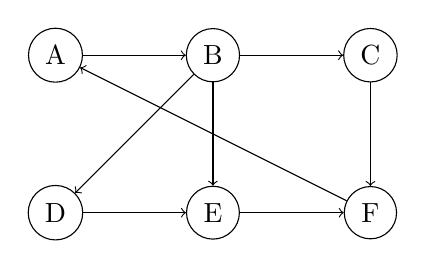
\begin{tikzpicture}[node distance=2cm]
    \node[circle, draw] (A) {A};
    \node[circle, draw, right of=A] (B) {B};
    \node[circle, draw, right of=B] (C) {C};
    \node[circle, draw, below of=A] (D) {D};
    \node[circle, draw, right of=D] (E) {E};
    \node[circle, draw, right of=E] (F) {F};

    \draw[->] (A) -- (B);
    \draw[->] (B) -- (C);
    \draw[->] (B) -- (D);
    \draw[->] (B) -- (E);
    \draw[->] (C) -- (F);
    \draw[->] (D) -- (E);
    \draw[->] (E) -- (F);
    \draw[->] (F) -- (A);
\end{tikzpicture}

\begin{parts}

\part[3]  Give the adjacency list for the graph. You should write the node in alphabetical order. (Leave it blank if the node has no neighbour)

\begin{align*} % Your solution here
    adj(A) =& [\underline{\qquad\qquad}],\\
    adj(B) =& [\underline{\qquad\qquad}],\\
    adj(C) =& [\underline{\qquad\qquad}],\\
    adj(D) =& [\underline{\qquad\qquad}],\\
    adj(E) =& [\underline{\qquad\qquad}],\\
    adj(F) =& [\underline{\qquad\qquad}],\\
\end{align*}


\part[3] Give the visited node order using the above adjacency list for Breadth First Search.
\begin{solution}
    
\end{solution}

\part[3] Give the visited node order using the above adjacency list for Depth First Search.
\begin{solution}
    
\end{solution}

\end{parts}

\raggedright
\titledquestion{DFS went wrong!}[6]
The following algorithm which runs DFS on a directed graph, but it contains a fatal error.
\begin{lstlisting}
    Create a stack.
    Choose the initial vertex and mark it as visited.
    Put the initial vertex onto the stack.
    while the stack is not empty:
        Pop a vertex V from the top of the stack.
        for each neighbor of V:
            if that neighbor is not marked as visited:
                Mark that neighbor as visited.
                Push that neighbor onto the stack.
\end{lstlisting}

    
Please give a graph as an counterexample and briefly explain why this algorithm is wrong. 
\\
\textit{Note: In this problem, we say a node is ``visited" whenever it is marked as visited. Pay special attention to how this method differs from the standard DFS in terms of the order in which nodes are marked as visited.}\\


\raggedright
\begin{solution}
    \vspace{200pt}
\end{solution}

\titledquestion{Friend or enemy?}[6]
\raggedright
Consider a set of \( n \) individuals, each of whom can have two types of relationships with others: friendship and enmity. It is also possible for individuals to have no relationship at all, or even to be both friends and enemies simultaneously. The relationships satisfy the following properties:

\begin{enumerate}
    \item If person \( a_i \) is a friend of person \( a_j \), then person \( a_j \) is also a friend of person \( a_i \) (friendship is symmetric).
    \item If person \( a_i \) is an enemy of person \( a_j \), then person \( a_j \) is also an enemy of person \( a_i \) (enmity is symmetric).
    \item Friends of friends are also considered friends. That is, if person \( a_i \) is a friend of person \( a_j \) and person \( a_j \) is a friend with person \( a_k \), then person \( a_i \) is a friend of person \( a_k \).
    \item Enemies of enemies are considered friends. That is, if person \( a_i \) is an enemy of person \( a_j \) and person \( a_j \) is an enemy of person \( a_k \), then person \( a_i \) is a friend of person \( a_k \).
\end{enumerate}

Given a set of relationships represented as:

\begin{itemize}
    \item A set of friendship pairs \( F \subseteq \{(a_i, a_j) \mid 1 \leq i, j \leq n, i \neq j\} \)
    \item A set of enmity pairs \( E \subseteq \{(a_i, a_j) \mid 1 \leq i, j \leq n, i \neq j\} \)
\end{itemize}

\textbf{Your task is to determine the number of distinct groups that can be formed, where each group consists of individuals who are all friends with each other.} (When forming groups, we do not need to consider enemy relationships.)

You should ensure that your algorithm has a time complexity of $O((m+n)\alpha(n))$, where $m$ is $|F|+|E|$ and $n$ is the number of individuals, but no proof is required.

\textit{Hint: You may consider representing each individual as two nodes: one for their friendships and one for their enmities. Utilize the disjoint set to efficiently manage and merge these relationships.}

\raggedright
\begin{solution}
\vspace{150pt}

\end{solution}

\end{questions}

\end{document}